% !TeX root = ../main.tex

\section{Verwendung}

Im folgenden Abschnitt wird ein Beispiel erläutert, bei dem die meisten Funktionalitäten des Projektes getestet werden können.

Zunächst muss ein Schachbrett bereitgestellt werden, bei dem ein Feld jeweils \mbox{$6\times6$~cm} bis \mbox{$7\times7$~cm} groß ist. Somit wird garantiert, dass sich die Dezibots komfortabel bewegen und rotieren können. Auf dem Dezibot $D$, welcher eine Schachfigur simulieren soll, muss für die Demonstration das \texttt{examples/""showcase/""embedded\_\allowbreak chess\_\allowbreak piece.ino}\footnote{\url{https://github.com/embedded-chess/embedded-chess-pieces/blob/main/example/EmbeddedChessPieces/examples/showcase/embedded_chess_piece/embedded_chess_piece.ino}} Programm $P_D$ installiert werden. Für dieses Beispiel ist ein druckbares Schachbrett im Repository der Dokumentation unter \texttt{assets/""showcase\_\allowbreak boards.pdf}\footnote{\url{https://raw.githubusercontent.com/embedded-chess/doc/refs/heads/main/assets/showcase_boards.pdf}} abgelegt.

Ein weiterer Dezibot muss als \emph{Beacon} $B$ agieren. Dieser sendet ein Infrarot"=Signal aus, um die Rotation eines Dezibots zu regeln (vgl. \autoref{sec:movement-ir}). Dafür muss auf diesem \texttt{examples/""beacon.ino}\footnote{\url{https://github.com/embedded-chess/embedded-chess-pieces/blob/main/example/EmbeddedChessPieces/examples/beacon/beacon.ino}} $P_B$ installiert werden.

Wie in \autoref{fig:usage} angedeutet ist, muss $B$ außerhalb des Schachbretts platziert und ungefähr in die Mitte des Schachbretts ausgerichtet werden. $D$ muss auf jenem Feld platziert werden, welches in $P_D$ festgelegt wurde. Eine weiße Figur muss dabei in Richtung Norden zeigen, eine schwarze in Richtung Süden. Die Richtungen sind aus dem in \autoref{fig:usage} dargestellten Kompass zu entnehmen.

\begin{figure}[h]
    \centering
    \begin{subfigure}[c]{0.49\textwidth}
        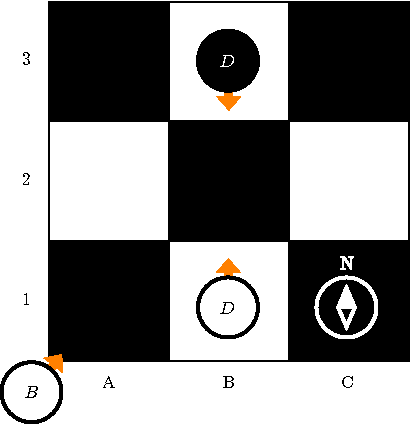
\includegraphics[width=\textwidth]{../assets/usage.drawio.pdf}
    \end{subfigure}
    \hspace{0.5em}
    \begin{subfigure}[c]{0.47\textwidth}
        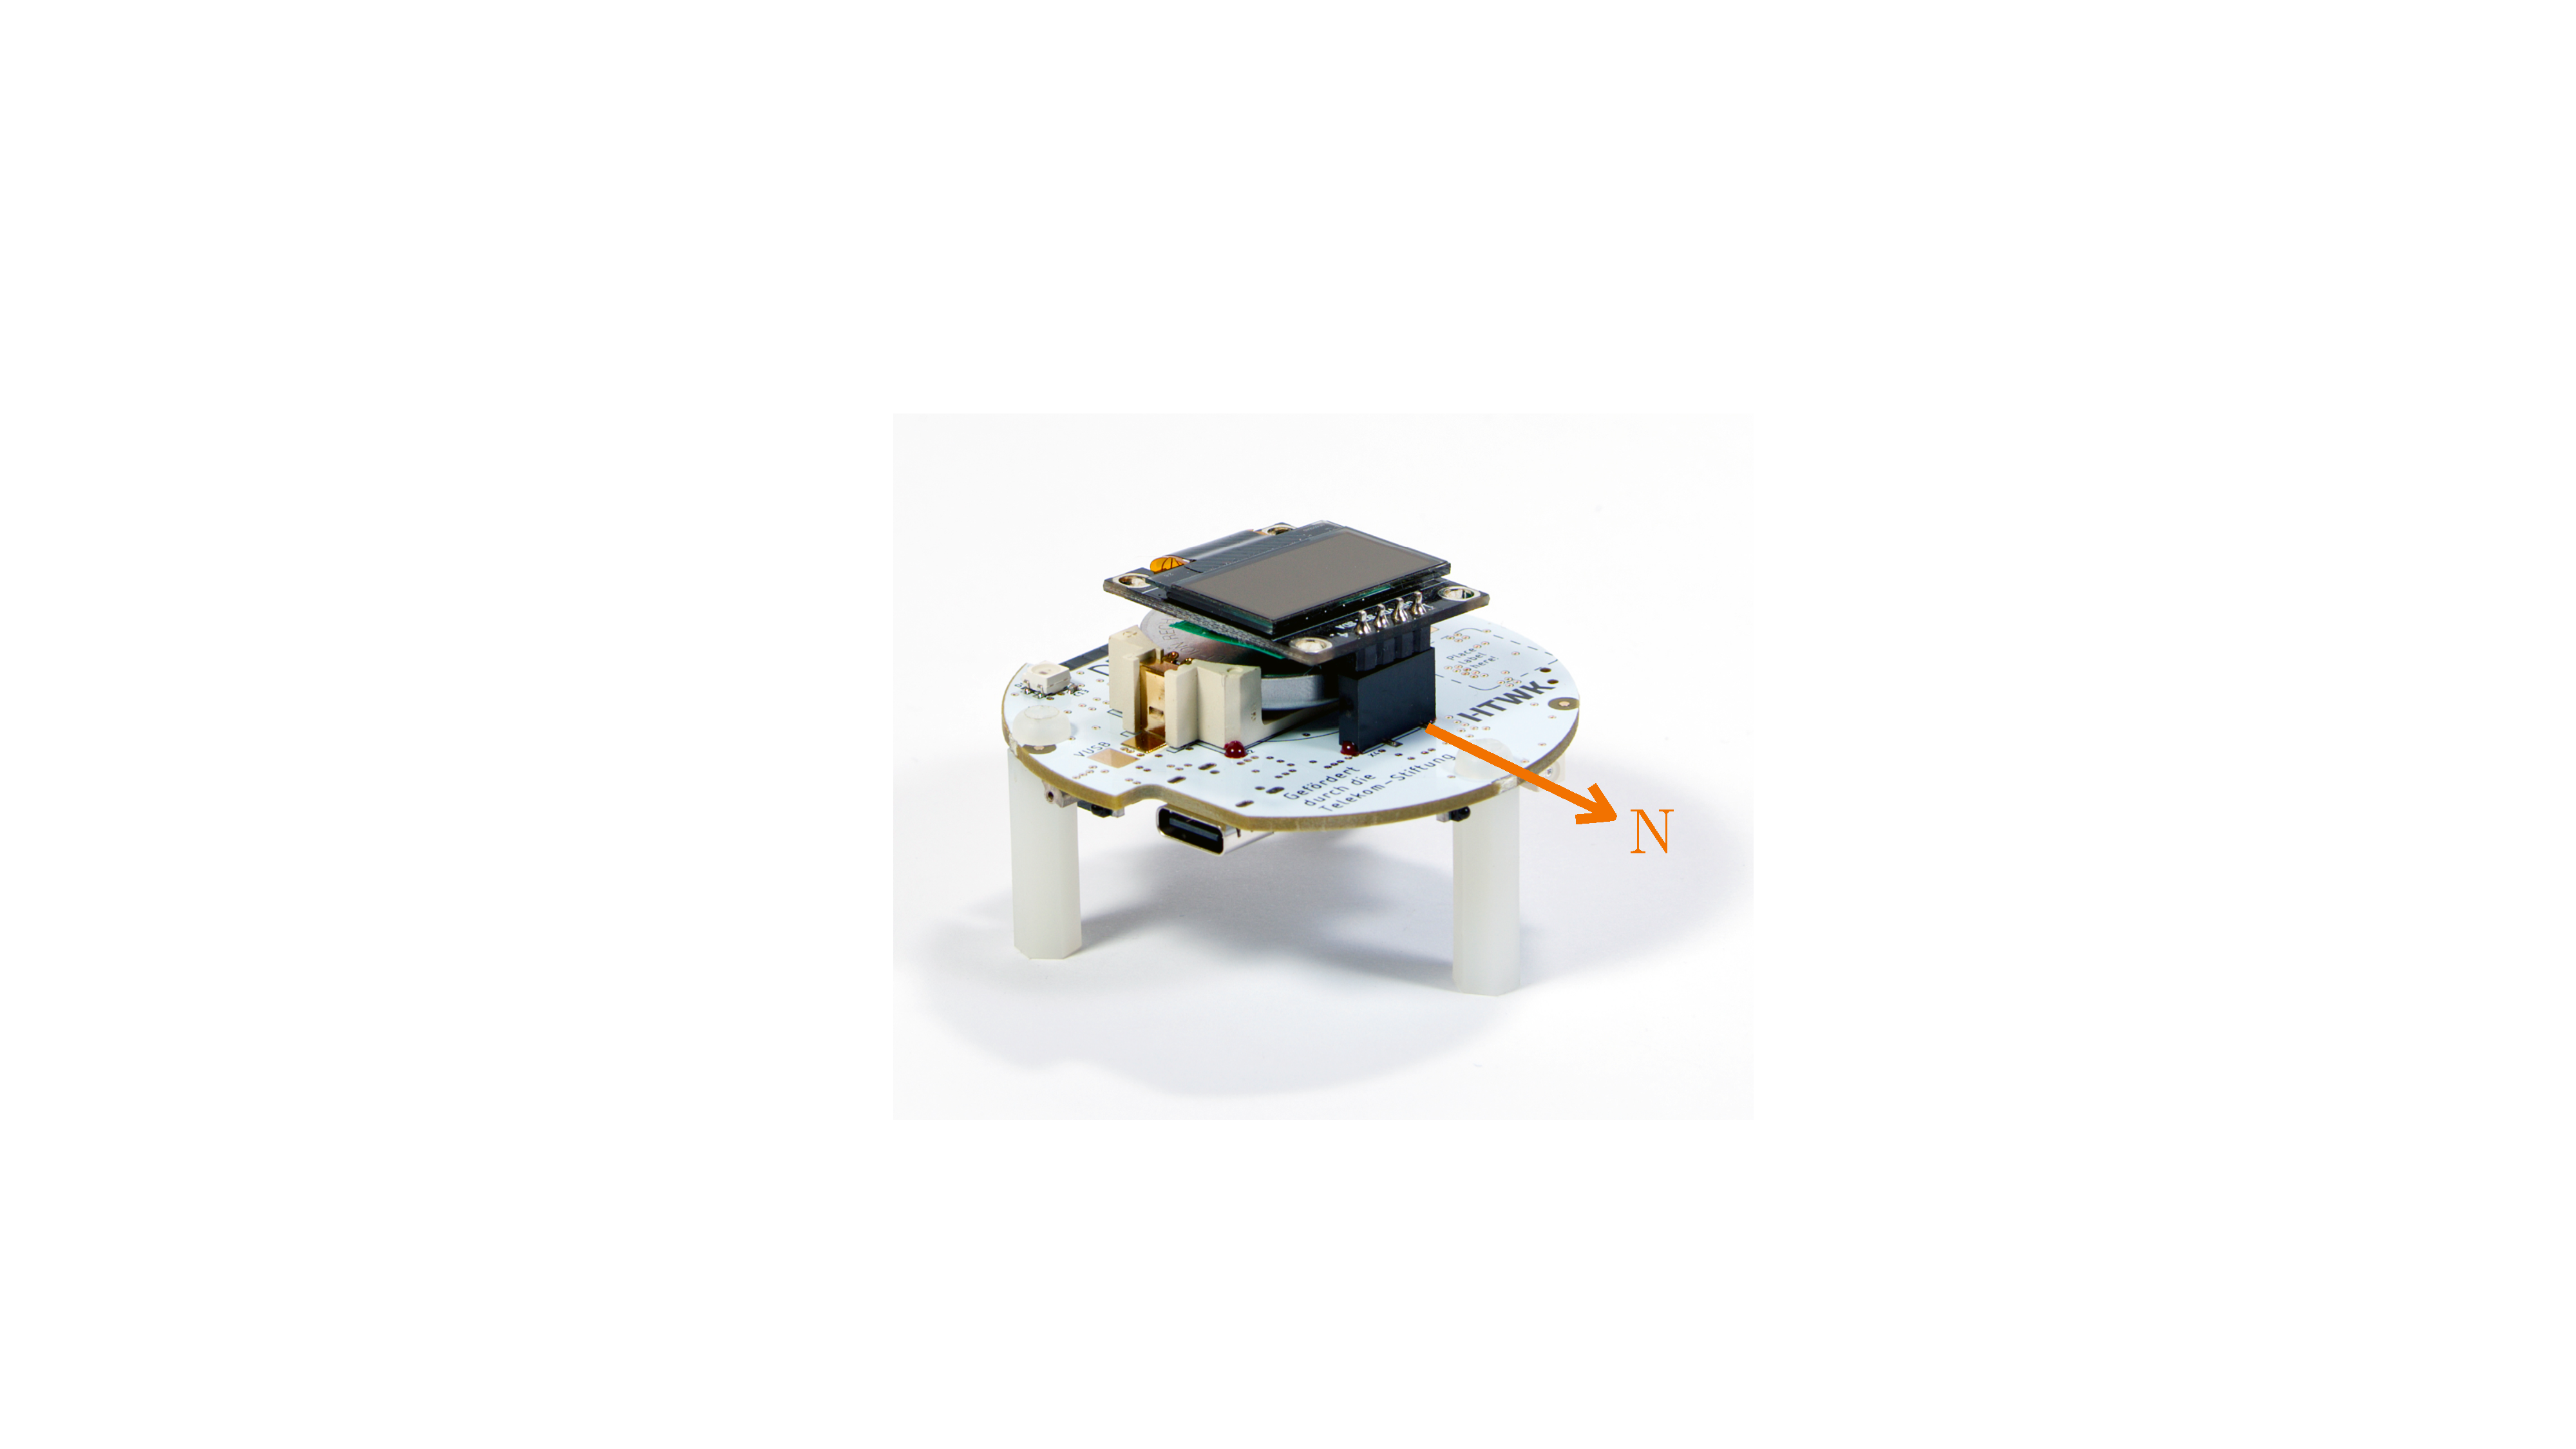
\includegraphics[width=\textwidth]{../assets/dezibot_total_view_north.png}
    \end{subfigure}
    \caption{Links: Ausschnitt eines Schachbretts, auf dem zwei Dezibots ($D$) dargestellt sind, welche eine weiße bzw. schwarze Figur simulieren. Unten links ist ein dritter Dezibot dargestellt, welcher als Beacon ($B$) agiert. In orange sind die Ausrichtungen der jeweiligen Dezibots angedeutet, welche rechts mit einem physikalischen Dezibot verdeutlicht wird. Dabei zeigt der rote Pfeil in Richtung Norden (Verwendung des speziell entworfenen 3D-gedruckten Modells~\cite[vgl.][]{felttipDezibotAlignmentPointer2025}).}
    \label{fig:usage}
\end{figure}

Zu Beginn des Beispiels wird eine Kalibrierung der Infrarot"=Messung durchgeführt, um die Erkennung der Feldfarben (schwarz / weiß) zu verbessern (vgl.~\autoref{sec:colour-calibration-ir}). Dafür muss der Dezibot $D$ zunächst auf ein weißes und anschließend auf ein schwarzes Feld platziert werden. Eine entsprechende Aufforderung wird auf das Display des Dezibots gedruckt (vgl.~\autoref{fig:colour-calibration-display-print}). Falls dabei störende Infrarot"=Signale gemessen wurden, werden die Spielenden dazu aufgefordert, diese zu entfernen (vgl.~\autoref{fig:display-interfering-ir}). Eine Quelle kann der Beacon sein. Daher wird empfohlen, diesen nur zu aktivieren, wenn $D$ dazu über sein Display auffordert (vgl.~\autoref{fig:display-no-ir-signal}). Falls nach dem Ausschalten des Beacons die Warnung immer noch auftritt, sollten die Signale anderer Infrarot"=Quellen, wie bspw. der Sonne, entfernt werden.

Nach der Kalibrierung wird ein weißer Bauer (\emph{Pawn}) simuliert. Damit die Spielenden wissen, wie der Dezibot platziert werden muss, wird das initiale Feld sowie die erwartete Ausrichtung auf das Display gedruckt. Anschließend validiert die Figur verschiedene Züge. Falls diese ungültig sind, wird ein rotes Lichtsignal ausgegeben und der Zug verworfen. Andernfalls leuchtet der Dezibot kurz grün und startet seine Bewegung. Nach Abschluss der vordefinierten Züge, wird eine schwarze Königin (\emph{Queen}) analog, allerdings mit anderen Zügen, simuliert. Der Wechsel der Figur ist auf dem Display zu erkennen.

Zum weiteren Ausprobieren wurde der \texttt{examples/""playground/""playground.ino}"=Sketch\footnote{\url{https://github.com/embedded-chess/embedded-chess-pieces/blob/main/example/EmbeddedChessPieces/examples/playground/playground.ino}} erstellt, bei dem die einzelnen Einstellungsmöglichkeiten genauer erläutert sind. Dort können die zu simulierende Figur, die auszuführenden Züge sowie weitere Kalibrierungsoptionen eingestellt werden.
